\chapter{Resultados  Preliminares}
\label{chap:resultados_discussao}

Os testes iniciais foram aplicados ao conjunto de dados do \gls{ACDC}. Este conjunto de dados público já vem separado com 100 exames para treino e 50 para testes. A Figura \ref{fig:fig018} e \ref{fig:fig019} são exemplos de imagens de \gls{DCM} e \gls{HCM} capturadas na diástole com suas respectivas máscaras. Na Figura \ref{fig:fig020} temos uma imagem de coração em estado sem anomalia (\gls{NOR}). As imagens demonstradas fazem parte do conjunto de treinamento.

\begin{figure}[h!]
    \centering
    \caption{Captura Diastólica CMD}
    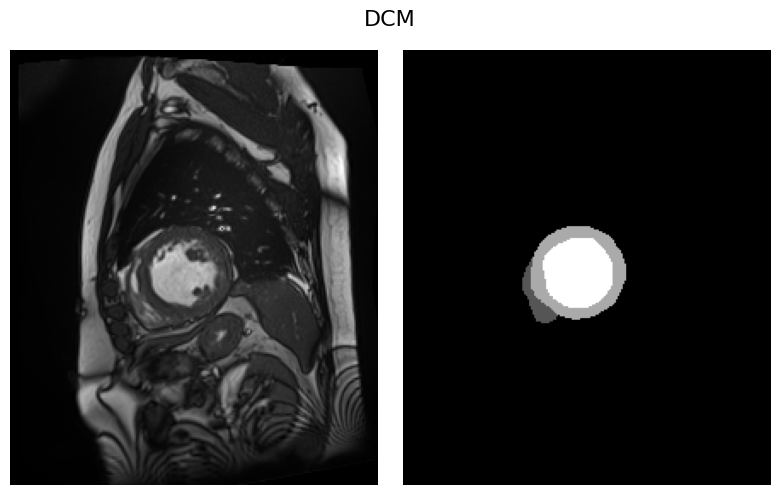
\includegraphics[width=0.65\textwidth]{figures/fig018.png}
    \caption*{Fonte: Autor}
    \label{fig:fig018}
\end{figure}

\begin{figure}[h!]
    \caption{Captura Diastólica de CMH}
    \centering
    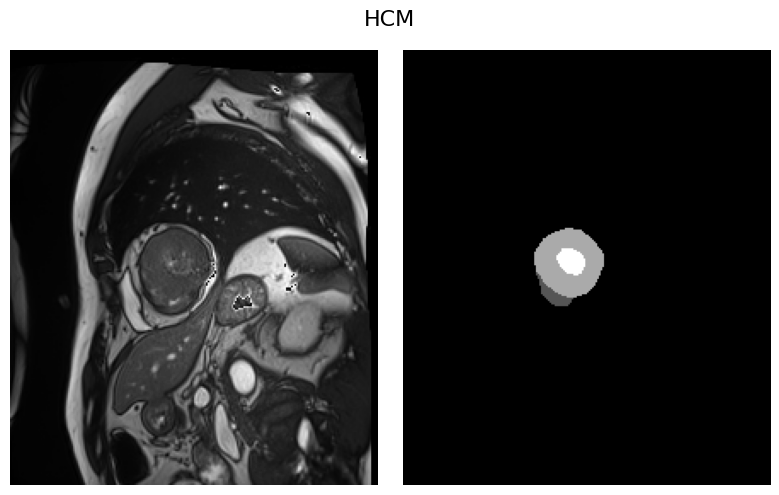
\includegraphics[width=0.65\textwidth]{figures/fig019.png}
    \caption*{Fonte: Autor}
    \label{fig:fig019}
\end{figure}

\begin{figure}[h!]
    \centering
    \caption{Captura Diastólica NOR}
    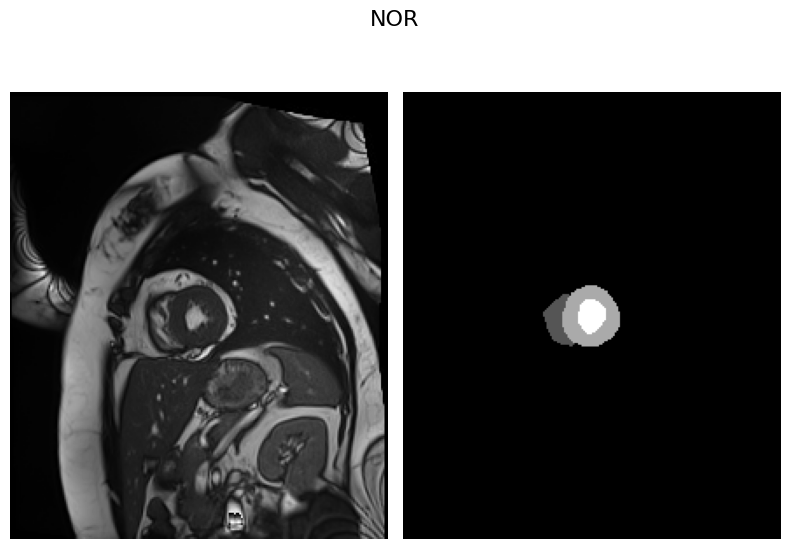
\includegraphics[width=0.65\textwidth]{figures/fig020.png}
    \caption*{Fonte: Autor}
    \label{fig:fig020}
\end{figure}

Os resultados foram obtidos aplicando a metodologia previamente apresentada, foram extraídas as características radiômicas e profundas, após foi aplicado o \textit{F-Test} para seleção de características e o resultado concatenado. Em seguida, o modelo de autoatenção foi aplicado, os hiperparâmetros utilizados são: taxa de aprendizado $\LR$, otimizador \gls{Adam} e aproximadamente $\Epochs$ épocas. Por fim, é aplicada a função matemática sigmoide e definido o limite de $0,5$ para corte onde os valores acima deste limite são classificados como \gls{CMH} e os demais como normal. As métricas resultantes podem ser conferidas na Tabela \ref{tab:metrics}. A matriz de confusão é apresentada na Figura \ref{fig:fig016} e um gráfico ilustrando da \gls{ROC} é apresentado na Figura \ref{fig:fig017}

\begin{table}[h!]
    \centering
    \caption{Métricas do Experimento}
    \renewcommand{\arraystretch}{1} % default é 1 
    \begin{tabular}{|c|c|}
    \hline 
          \textbf{Métrica} & \textbf{Valor} \\ 
    \hline 
        Acurácia & 0.62 \\ 
    \hline 
        Precisão & 0.67 \\ 
    \hline 
        Revocação & 0.10 \\ 
    \hline 
        AUC & 0.63 \\ 
    \hline 
    \end{tabular} 
    \caption*{Fonte: Autor}
    \label{tab:metrics}
\end{table}

\begin{figure}[h!]
    \centering
    \caption{Matriz de Confusão}
    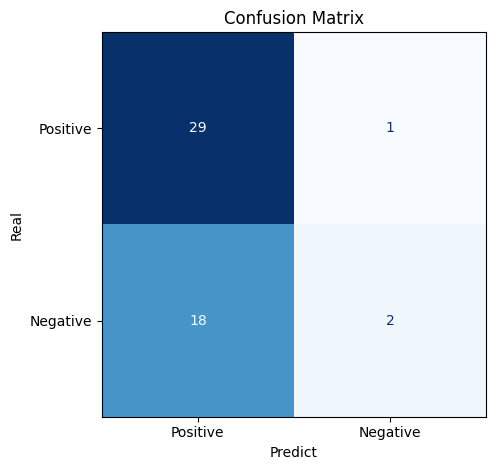
\includegraphics[width=0.55\textwidth]{figures/fig016.png}
    \caption*{Fonte: Autor}
    \label{fig:fig016}
\end{figure}

\begin{figure}[h!]
    \centering
    \caption{ROC}
    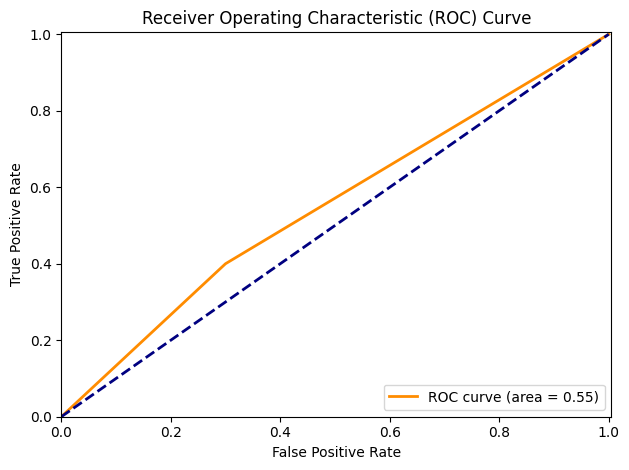
\includegraphics[width=0.75\textwidth]{figures/fig017.png}
    \caption*{Fonte: Autor}
    \label{fig:fig017}
\end{figure}

%--------------------------------------------------------
\section{Considerações Finais do Capítulo} 
\label{sec:cap6_consideracoes_finais}

Os resultados obtidos, aplicando a arquitetura proposta por \citeonline{aiSelfAttentionBasedFusion2023} com modificações na quantidade de características utilizadas e aplicado em imagens de \gls{RMC} para identificação de cardiomiopatias, em contraste com o trabalho mencionado que foi aplicado à identificação de câncer no pulmão, obteve resultados menos relevantes que o original. Isto indica que há espaço para exploração e melhorias a serem proposta para o âmbito de cardiomiopatia. Algumas, abordagens ainda são tidas em vista como manipular o seletor de características e a sua quantidade, testar novos hiperparâmetros para os modelos, ao invés de ter um único módulo de autoatenção, aplicar vários em cascata, etc.

